\documentclass{article}
\usepackage[utf8]{inputenc}
\usepackage{graphicx}
\usepackage{indentfirst}
\usepackage{amsmath}

\edef\restoreparindent{\parindent=\the\parindent\relax}
\usepackage{parskip}
\restoreparindent


\title{A Model for Supply Allocation in the City of Vancouver to Prepare for a Natural Disaster}
\author{Gareth Anonby, Ashutosh Dubal,\\ Lacey Liang, Reece McGowan\\\\
Department of Mathematics, Simon Fraser University, Burnaby, BC, Canada}

\date{}

\usepackage[a4paper, total={6in, 8in}]{geometry}


\begin{document}

\maketitle

\

\begin{abstract}
     This paper aims to outline a supply plan that outfits 25 support hubs in the City of Vancouver with essential food and water supplies in the event of a natural disaster. We propose a model that takes as input the population, population distribution, percentage of population that requires assistance, number of days to supply, number of cans and bottles per day, Costco weekly capacity constraints, cost of gas per kilometre for the chosen vehicle, and carrying capacity of chosen vehicle. The model then proposes a supply plan that outfits the hubs with the necessary amount of supplies at the least cost in the least amount of time. 
\end{abstract}

\newpage

\section{Introduction}

\indent The City of Vancouver is currently faced with a daunting reality. According to some experts, there is a 12\% probability that a magnitude-9.0 earthquake  will strike near the West Coast in the next 50 years, causing massive damage and displacing thousands of people from their homes. The best way to ensure the smallest loss of life is to be prepared. This paper aims to outline a plan for 25 existing support hubs in the City of Vancouver to ensure each of them has an adequate amount of food and water to sustain those who might need assistance. The plan will consist of quantities of canned goods and water to buy from 3 Costcos in the City of Vancouver, as well as the best way to send these goods to 25 support hubs. The goal is to ensure the city has fully stocked shelters in the event of a natural disaster, such as an earthquake. We also recommend a plan to account for food spoilage and water expiration.

There are many operations research papers related to disaster relief. For example, Gutierrez et al. created a model that chooses the best location of a temporary relief center ``in order to optimize the delivery of relief goods to the randomly dispersed evacuation centers.''\cite{humanitariansupplychain} As well, Hall et al. proposed a model for ``scheduling costs and constraints within the manufacturer's capacity allocation problem.''\cite{supplyallocation} Our hope is to propose a model for the purposes of disaster preparation, while allowing the City of Vancouver to account for growing population in the future for this supply allocation problem. 

\section{Assumptions}

We're assuming the population and population distribution of Vancouver does not increase significantly over the course of our plan, which is approximately 3 years.  We are assuming the food and water has been processed according to USDA standards, and as such have a maximum shelf life \cite{can life}. Humans can survive for a number of weeks without food \cite{21daysnofood}, so we are assuming that 2 cans per day is a reasonable amount for comfort and sustainability for a week. We are also assuming that the support hubs are large enough to hold all of the cans of food and water bottles. 

\section{Model}

\subsection{Costco Location and Capacity}

We chose the following three Costco locations to utilize.

\begin{itemize}
    \item Costco #1 - 605 Expo Boulevard
    \item Costco #2 - 9151 Bridgeport Road
    \item Costco #3 - Willingdon Warehouse, 4500 Still Creek Drive
\end{itemize}

\begin{center}
    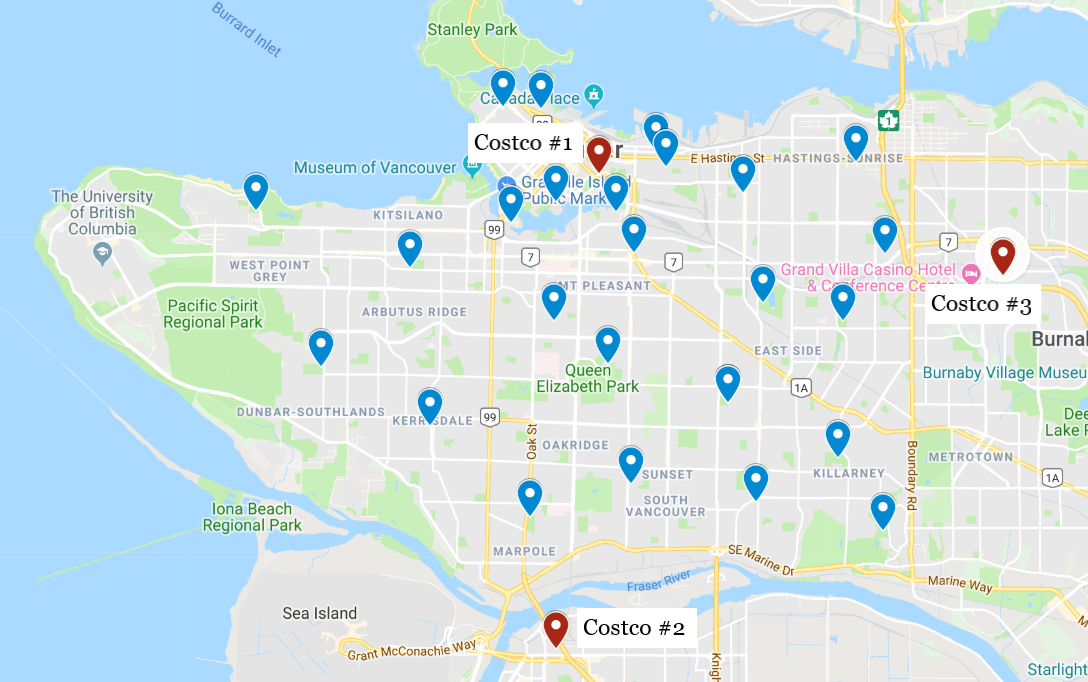
\includegraphics[scale=.3]{costcos.png}
    
    \caption{Figure 1: Costco Locations. Red denotes a Costco and blue denotes a support hub}
\end{center}

We chose these particular locations due to their proximity to the City of Vancouver. There is a 4th Costco located at 3550 Brighton Ave, Burnaby, BC, but we decided not to use this one due to its distance from the 25 support hubs. 

After consulting with Craig McGowan \cite{craig}, a Merchandise Manager at the Abbotsford Costco location, we were informed that purchasing 20,000 cans of pork and beans and 25,000 bottles of water per week is doable for a single Costco. This number could potentially change after entering discussions with Costco corporate, but the optimal solution will scale with the new quantities.

\subsection{Support Hub Population and Demand}

There are 25 support hubs as designated by the municipality of Vancouver that are to be used as places where citizens can ``gather to coordinate your efforts and offer assistance to other members of your community'' \cite{Vancouver.ca}.
Using the map provided on the \textit{Disaster Support Hubs} webpage \cite{Vancouver.ca}, we created boundaries around each support hub denoting the area of people that would likely use that particular hub, as shown in \textbf{Figure 2}. Each of the numbers represents one of the twenty-five support hubs found on the disaster support hubs map.

\begin{center}
    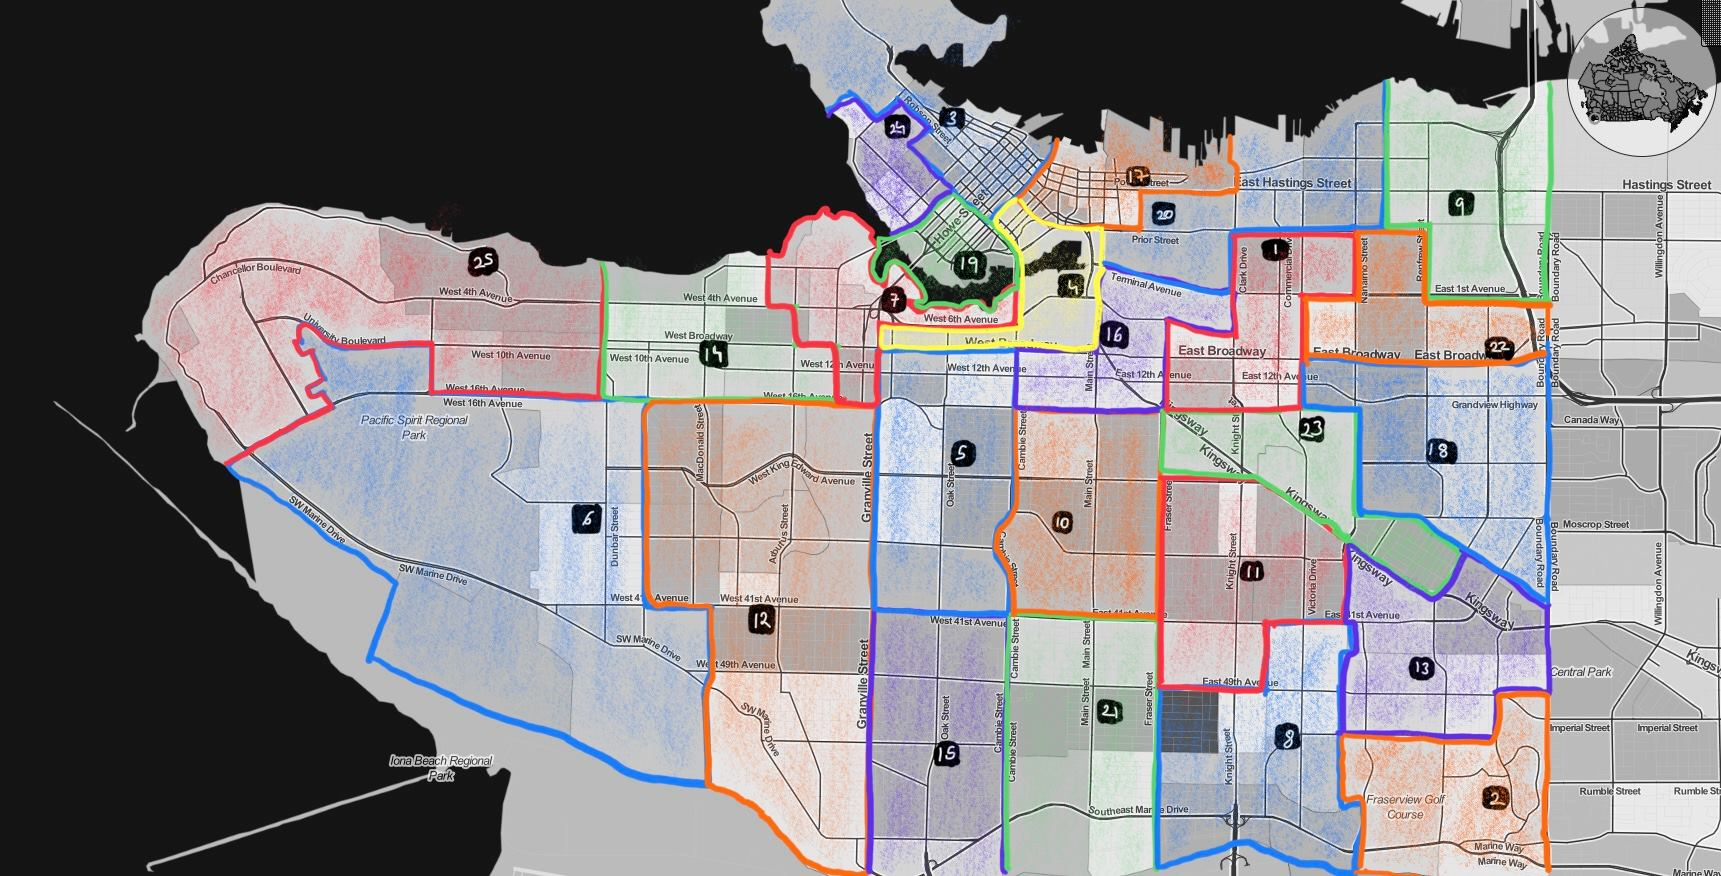
\includegraphics[scale=.25]{map_25_chunks.jpg}
    \caption{Figure 2: 25 Support Hub Chunks}
\end{center}

Using Census Mapper \cite{censusmapper}, we were able to calculate the population associated with each of these 25 blocks. Those numbers are shown here. 

\begin{center}
    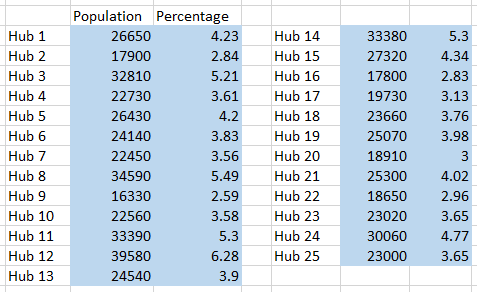
\includegraphics[scale=0.5]{hub_populations.png}
    
    \caption{Figure 3: Support Hub Populations}
\end{center}

Summing up these 25 chunks, we get a total population of 630,000 people. This is a slight simplification, however, as Census Mapper has their numbers in units of 100. The true number is 631,490, so we believe this number is close enough. We're going to assume that half of the people in a chunk need 2 cans per day for 7 days. Not everyone will need assistance, and we believe 50\% of citizens requiring assistance is an overestimate. This leaves us with the following calculations for cans.

\[(\frac{630,000 \;\text{people}}{2}) (\frac{2 \;\text{cans}}{1 \;\text{day}}) (7\;\text{days}) = 4,410,000\;\text{cans}\]

So we have a total of 4,410,000 cans. We will be using a timeline that fully utilizes the capacity of the Costcos. We believe it is in Vancouver's best interest to supply the support hubs in the shortest time possible in the off chance a natural disaster hits sooner than expected. The calculation for weeks, then, is as follows.

\[\frac{4,410,000\;\text{cans}}{60,000\;\text{cans per week}} = \text{73.5 weeks}\]

So 74 weeks was chosen because it almost fully utilizes the capacity of the Costcos. This number will be spread across all 25 support hubs depending on their relative percentage to the total population. That calculation is as follows.

\[\frac{\text{Population of chunk i}}{630,000 \;\text{people}} = \text{Percentage of total population for chunk i} = r_{i}\]

\[(4,410,000\;\text{cans})(r_{i}) = \text{Total cans required at support hub i} = c_{i}\]

\[\frac{c_i}{74\;\text{weeks}} = \text{Total demand of cans per week} = cw_i\]

\[\text{Where} \;i\in(1,...,25)\]

A sample calculation for support hub 1 looks like this.

\[\frac{26,650\;\text{people in support hub 1}}{630,000\;\text{people}} = 0.0423015873 = r_1\]

\[(4,410,000\;\text{cans})(r_1) = 186,550\;\text{cans required at support hub 1} = c_1\]

\[\frac{c_1}{74\;\text{weeks}} = 2520.945946\;\text{cans per week}\]

Which is then rounded down to 2520 cans per week for support hub 1. The World Health Organization recommends 2.5L per person per day in a natural disaster \cite{WHO}. The total demand for water, then, is as follows.

\[(\frac{2500\;\text{mL}}{\text{1 person per day}})(7\;\text{days})(315,000 \;\text{people}) = 5,512,500,000\;\text{mL}\]

Each bottle we would be purchasing from Costco holds 500mL, so we get the following number of bottles.

\[(5,512,500,000\;\text{mL})(\frac{1\;\text{bottle}}{500\;\text{mL}}) = 11,025,000\;\text{bottles}\]

Each Coscto can supply 25,000 bottles of water per week, so the timeline can be calculated as follows.

\[\frac{11,025,000\;\text{bottles}}{75,000\;\text{bottles per week}} = 147\;\text{weeks}\]

This number of weeks is on top of the 74 weeks for cans, so the City of Vancouver can either execute both plans together for 74 weeks, then deliver solely water for the remaining 73 weeks, or they can do the plans one after the other for a total of 221 weeks. We can find the demand for water bottles with a process similar to cans. A sample calculation for support hub 2 is shown as follows. 

\[\frac{17,900\;\text{people in support hub 2}}{630,000\;\text{people}} = 0.0284126984 = r_2\]

\[(11,025,000\;\text{bottles of water})(r_2) = 313,250\;\text{bottles of water required at support hub 2} = b_2\]

\[\frac{b_2}{147\;\text{weeks}} = 2130.95238\;\text{bottles of water per week at support hub 2}\]

This number is then rounded down to 2130. The demand per week for food and water is shown in \textbf{Figure 6}.

\subsection{Route costs}

We are basing our calculations on a standard 2019 Toyota Tacoma pickup truck. The fuel efficiency of this truck is 12.1L per 100km \cite{fuelconsumptionguide}. We are using the current gas price at time of writing at \$1.50 per litre. Of course, the gas price will likely be different when this plan is enacted, but the difference will be applied equally to all route costs, and will therefore not affect our final solution. The route calculation is performed as follows.

\[(\frac{12.1\text{L}}{100\;\text{km}})(\frac{\$1.50}{1\text{L}}) = \frac{\$0.1815}{\text{km}}\]

We increase this number by 10\% to account for the extra weight associated with carrying the goods.

\[(\frac{\$0.1815}{\text{km}})(1.10) = \frac{\$0.19965}{\text{km}}\]

Which we round to \$0.2 per kilometre. The cost for route i is calculated as follows.

\[(\frac{\$0.2}{\text{km}})(\text{distance of one-way trip for route i})(2) = \text{Cost of round trip for route i}\]

\begin{center}
 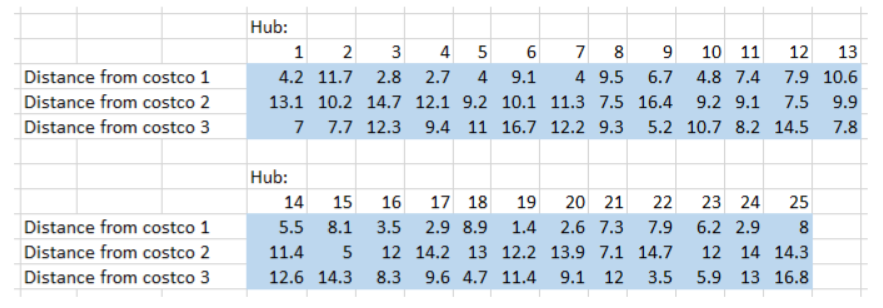
\includegraphics[scale=0.5]{distances.png}
 
 \caption{Figure 4: One-way distances for each support hub}
\end{center}

The standard carry load of a 2019 Toyota Tacoma is 1175 pounds \cite{toyotatacoma}. A can of food and a bottle of water each weigh roughly 1 pound. To avoid overloading, we are going to assume the trucks would be loaded with 1000 cans of food or 1000 bottles of water. We can then divide the calculated cost by 1000 to get an average cost per unit, shown in \textbf{Figure 5}. 

\subsection{Formulation}

\subsubsection{Decision Variables}
We are sending from 3 Costcos (\(C_i,i\in\!I,I=[1,3]\)) to 25 support hubs (\(H_j, j\in \!J, J=[1,25]\)). Note that \(C_1\) corresponds to the Costco at 605 Expo Blvd, \(C_2\) to the Costco at 9151 Bridgeport Road, and \(C_3\) to the Costco at Willingdon Warehouse, 4500 Still Creek Drive.
\\\\
\indent Our decision variables are \(f_{ij}\) and \(w_{ij}\). \(f_{ij}\) represents how many cans of food to send from \(C_i\) to \(H_j\) per week. And \(w_{ij}\) represents how many bottles of water.

\subsubsection{Objective Function}
Our objective is to minimize the cost of supplying each support hub. To do that, we need the cost per can of food sent from \(C_i\) to \(H_i\), \(a_{ij}\). And the cost per bottle of water, \(b_{ij}\). The values of \(a_{ij}\) can be seen here.

\begin{center}
    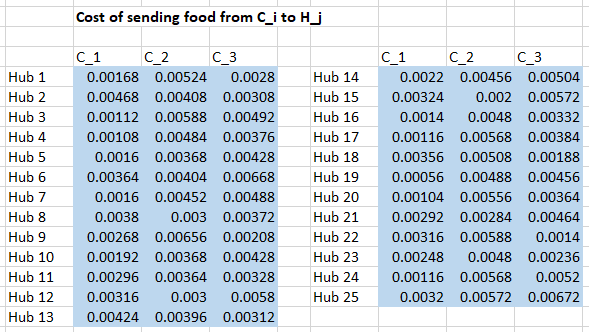
\includegraphics[scale=.4]{cost_from_ci_to_hj.png}
    
    \caption{Figure 5: Cost per unit for each of the 75 routes}
\end{center}



\noindent
Note that due to having the same truck capacity, the values of \(b_{ij}\) are the same as the values of \(a_{ij}\). 
\\\\
\indent \(a_{ij}f_{ij}\) equals the weekly cost of sending food from \(C_i\) to \(H_j\). Adding the costs for each possible route gives our total weekly cost to supply each support hub. The number of weeks we plan to supply food for, \(p\), is 74. And the number of weeks we plan to supply water for, \(q\), is 147. Multiplying the cost of food per week by the number of weeks we plan to supply for gives the total cost for supplying food. Doing the same with water gives the total cost for supplying water. Adding these give the total cost to supply the support hubs with enough food and water to last a week after a natural disaster.
\[T=p\sum_{i\in I} \sum_{j\in J} (a_{ij}f_{ij}) + q\sum_{i\in I} \sum_{j\in J} (b_{ij}w_{ij})\]




\subsubsection{Constraints}
Each support hub has a weekly demand for food and water. We will use the variables \(g_j\) and \(h_j\) to represent the weekly demand for food and water, respectively, at support hub j. The values of \(g_j\) and \(h_j\) can be seen here.




\begin{center}
    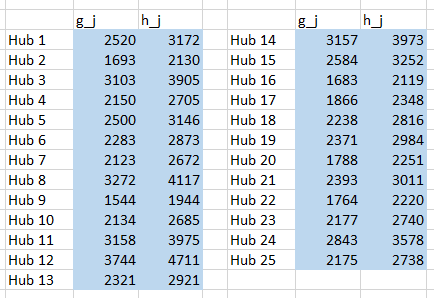
\includegraphics[scale=.4]{weekly_demand_for_food_and_water.png}
    
    \caption{Figure 6: Weekly demand for food and water}
\end{center}



We have the constraints that each support hub must get enough food and water to satisfy the weekly demand. This can be formulated as
\[\sum_{i\in I} f_{ij} \ge g_j\]
\[\sum_{i\in I} w_{ij} \ge h_j\]

Each Costco has a limit on how many cans and bottles you can buy per week. Therefore, we need to add constraints to ensure the amount of supplies bought from a given Costco do not exceed its capacity. Note that each Costco has the same capacity. The capacity for canned food is 20,000 cans per week, for water it is 25,000 bottles per week.
Now we can add the constraints here.
\[\sum_{j\in J} f_{ij}  \le 20000\]
\[\sum_{j\in J} w_{ij} \le 25000\]

\section{Results}

Running Solver in our Excel spreadsheet, we find the following supply plan for cans of food.

\begin{center}
    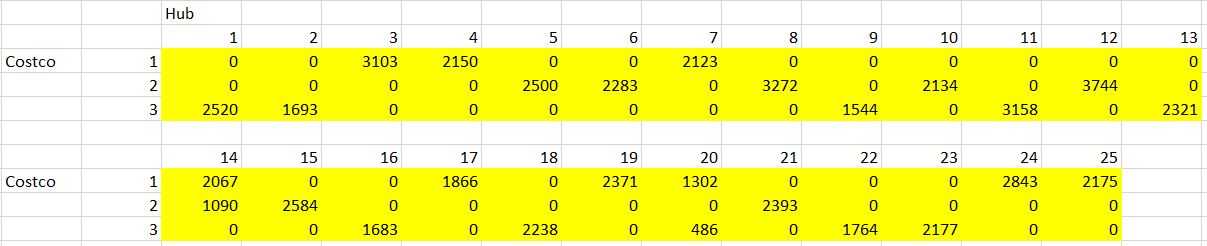
\includegraphics[scale=0.6]{food_plan_per_week_74_weeks.png}
    \caption{Figure 7: Cans of food per week for each route}
\end{center}

The total cost per week for food is \$145.38. We also find the following supply plan for bottles of water.

\begin{center}
    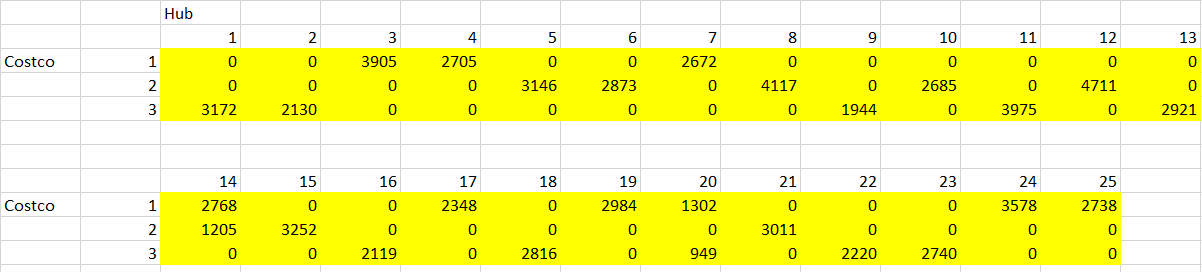
\includegraphics[scale=0.6]{water_plan_per_week_147_weeks.png}
    \caption{Figure 8: Bottles of water per week for each route}
\end{center}

The total cost per week for water is \$183.415. The total cost to deliver all materials is \$37,718.40.

\section{Discussion}

From our results, we find the following capacity constraints

\begin{table}[!h]
    \centering
    \begin{tabular}{c|c}
    Costco 1     & 20,000\\
        Costco 2 & 20,000 \\
        Costco 3 & 19,584
    \end{tabular}
    \caption{ Costco dispatch for food}
\end{table}

\begin{table}[!h]
    \centering
    \begin{tabular}{c|c}
    Costco 1     & 25,000\\
        Costco 2 & 25,000 \\
        Costco 3 & 24,986
    \end{tabular}
    \caption{Costco dispatch for water}
    \label{tab:my_label}
\end{table}

We notice that Costco 1 and Costco 2 are used to full capacity while Costco 3 has some remaining room. This is due to the fact that Costco 1 and 2 are closer to most of the support hubs than Costco 3, as seen in \textbf{Figure 1}. Intuitively, Solver looks at all the cheapest costs and fills as much demand as it can using these. Costco 1 and 2 are closest to the most support hubs, so naturally they hit their max capacity before Costco 3. The program chooses routes with low cost while also taking the demand into account, along with what the costs for the other Costcos routes are. Costco 1 has good connections but to fully utilize all of these routes, other Costcos would be forced to use worse routes. So, we end up with a mix of excellent routes and subpar routes. This pattern continues until eventually the capacities for Costco 1 and 2 are nearly full, and the program must split the remainder as best it can, leaving us with hubs 14 and 20 receiving supplies from multiple Costcos. In the case of support hub 20, we see that it is getting some supplies from Costco 3. The cost for this route is \$0.00364 per unit, which is still reasonable relative to the other costs.

We have formulated our model in such a way that supply equals demand. When we change the number of cans or water bottles, we also change the amount of weeks to match this. Essentially, we have a plan that scales with the amount of cans, bottles, or population you input. The cost may increase or decrease as the amount of cans change, but the same routes will be used. The model allows us to input the population, population distribution, percentage of population that requires assistance, number of days to supply, number of cans and bottles per day, Costco weekly capacity constraints, cost of gas per kilometre for the chosen vehicle, and carrying capacity of the chosen vehicle, with which the model will provide an optimal solution.

According to the USDA, one of the most important factors in the shelf life of canned foods is rust \cite{can life}. Also, bottled water has an indefinite shelf life \cite{bottledwaterindef}, but after enough time has passed the chemicals from the bottle can begin to seep into the water ruining the taste and potentially causing harm \cite{bottledwaterexp}. For these reasons, we are recommending a recurrent use of this plan. This particular plan, for example, could be executed over the course of 147 weeks, or just under 3 years. We believe 10 years is an appropriate amount of time to wait before replacing the canned food and water. So, 10 years after the first delivery, the City of Vancouver should input new values into the model and execute it. Each week, they should remove the oldest batch from each support hub and replace it with a new one. After this new plan has been enacted, each support hub will have a new supply that will be useable for roughly 10 years. This process should be repeated as long as the City of Vancouver wants to continue with this type of disaster preparation.

\subsection{Recommendations}

We have a few recommendations for improvement. Our model is currently based on a unit price per can/bottle, which we derive by taking the total cost of sending 1000 units and dividing it by 1000 to obtain an average cost per unit. This is not a bad representation of the problem, but it is also not an exceptional one. In reality, our purchasing costs are fixed. The only variable cost is how many truck loads we send. For example, if we were to send 1500 cans on a route, a single truck would need to perform three one-way trips. It would fill up with 1000 cans at a Costco, travel to the support hub, drop off the cans, travel back to the Costco, fill up with the remaining 500 cans, and make one final trip to the support hub. This means the route was used three times, and this is where our cost comes from. This cost will hold so long as the number of cans on a route is within the interval [1000, 1999). We came up with an Excel function for this.

\[=c_i*(CEILING(x_i/1000)*2-1))\]

Where c\textsubscript{i} represents the cost to drive route i and x\textsubscript{i} represents the amount of cans on route i. The objective function would then be to minimize the sum of all these values. Unfortunately, using this formula creates a non-linear objective function, forcing us to use the GRG Non-linear solver in Excel's solver. Using this solver gave us non-optimal answers and implementing the CEILING function in a linear fashion requires more constraints than Solver can handle, as we would need 103 constraints. Another option would be to use a different program such as AMPL. Due to time constraints, we could not learn the syntax necessary to translate our model into AMPL. We also chose 50\% of the population, but we believe this may be an overestimate. A better estimate would require a comprehensive scenario analysis, which would inform the city how many people will actually need to use these support hubs. Making these improvements should create a more accurate model.




\newpage
\begin{thebibliography}{9}

\bibitem{humanitariansupplychain}
Gutierrez, & Mutuc. (2018). A Model for Humanitarian Supply Chain: An Operation Research Approach. Procedia Engineering, 212, 659-666.

\bibitem{supplyallocation}
Capacity Allocation and Scheduling in Supply Chains. (2010). Operations Research, 58(6), 1711-1725.

\bibitem{Vancouver.ca} 
(2019). \textit{Disaster support hubs}. City of Vancouver. [Online]. Available:
\\\texttt{https://vancouver.ca/home-property-development/disaster-support-hubs.aspx}. [March 7, 2019]

\bibitem{censusmapper}
(February 25, 2019). \textit{Population Density of Vancouver (Canada Census 2016)}. Census Mapper. [Online]. Available:
\\\texttt{https://censusmapper.ca/maps/1493#12/49.2445/-123.1773}. [March 19, 2019]

\bibitem{WHO}
Brian Reed and Bob Reed. \textit{How much water is needed in emergencies.} World Health Organization. [Online]. Available: 
\\\texttt{https://www.who.int/water\_sanitation\_health/publications/2011/tn9\_how\_much\_water\_en.pdf}. [March 25,2019]

\bibitem{can life}
(August 2014). \textit{Shelf-Stable Food Safety}. United States Department of Agriculture Food Safety and Inspection Service. [Online]. Available: 
\\\texttt{https://www.fsis.usda.gov/wps/wcm/connect/77ffde83-dc51-4fdf-93be-}
\\\texttt{048110fe47d6/Shelf\_Stable\_Food\_Safety.pdf?MOD=AJPERES}\newline[March 25,2019]

\bibitem{21daysnofood}
Alan D. Lieberson. (November 8, 2004). \textit{How Long Can a Person Survive without Food?}. Scientific American. [Online]. Available: \texttt{https://www.scientificamerican.com/article/how-long-can-a-person-survive-without-food/}. [March 23, 2019]

\bibitem{craig}
McGowan, C. (March 23, 2019). Personal interview. Relative of Reece McGowan.

\bibitem{fuelconsumptionguide}
Natural Resources Canada. 2019. 2019 Fuel Consumption Guide. 43pp. Available: \\\texttt{https://www.nrcan.gc.ca/sites/www.nrcan.gc.ca/files/oee/pdf/transportation/tools}
\\\texttt{/fuelratings/2019\%20Fuel\%20Consumption\%20Guide.pdf?fbclid=IwAR3EBI-esvFeV27yBra0JF-}
\\\texttt{CUN3PJTACcS0aOHrGiVYG-SIIXaSsXh1FlLs}

\bibitem{toyotatacoma}
\textit{2019 Toyota Tacoma Full Specs}. Toyota. [Online]. Available: \\\texttt{https://www.toyota.com/tacoma/features/weights\_capacities/7594/7150/7582/7598}. [March 31, 2019]

\bibitem{bottledwaterindef}
Posnick, L. Sc.D, Kim, H. Ph.D. (September 2002). \textit{Bottled Water Regulation and the FDA}. Food Safety Magazine. [Online]. Available:
\\\texttt{https://www.foodsafetymagazine.com/magazine-archive1/augustseptember-2002/}
\\\texttt{bottled-water-regulation-and-the-fda/}
[March 28, 2019]

\bibitem{bottledwaterexp}
Radford, B. (June 9, 2010). \textit{Why Do Bottles of Water Have Expiration Dates?}. LIVESCIENCE. [Online]. Available:
\\\texttt{https://www.livescience.com/32636-why-do-bottles-of-water-have-expiration-dates-.html}.
[March 28, 2019]

\end{thebibliography}

\end{document}
